\setcounter{deso}{3}
\begin{name}
	{ÔN TẬP KIỂM TRA CUỐI HỌC KÌ 1}
	{TOÁN 10}
	{LỚP TOÁN THẦY PHÁT}
	{\thoigian}
\end{name}
%================================PHẦN I
\caulc
\Opensolutionfile{ans}[ans/0-HK1-KN-3-DoanThiDiem-HaNoi-2324-Phan-I]

\begin{ex}%[0-HK1-KN-3-DoanThiDiem-HaNoi-2324]%[VN-MT-6,VM032]%[0D1N3-3]
	Cho tập hợp $A=(-1;2)$; $B= [0;3]$. Khi đó, tập $A\cap B$ là
	\choice
	{\True $ [ 0;2)$}
	{$ (-1;3]$}
	{$ (-1;0)$}
	{$ [2;3]$}
	\loigiai{
		\begin{center}
			\begin{tikzpicture}[scale=1, font=\footnotesize, line join=round, line cap=round, >=stealth]
				\draw[-stealth] (-2,0)--(4,0);
				\path 
				(-1,0)node{$($} +(90:0.5) node{$-1$}
				(2,0) node{$)$} +(90:.5) node{$2$}
				(0,0) node{$[$} +(90:.5) node{$0$}
				(3,0) node{$]$} +(90:.5) node{$3$}
				; 
				\fill[opacity=0.6,pattern=north east lines] (-2,-4pt) rectangle (-1,4pt) (2,-4pt) rectangle (3.9,4pt);
				\fill[opacity=0.6,pattern=north west lines] (-2,-4pt) rectangle (0,4pt) (3,-4pt) rectangle (3.9,4pt);
			\end{tikzpicture}
		\end{center}
		Ta có $A\cap B=(-1;2)\cap [0;3]=[0;2)$.}
\end{ex}


\begin{ex}%[0-HK1-KN-3-DoanThiDiem-HaNoi-2324]%[VN-MT-6,VM032]%[0H9N2-1]
	Trong mặt phẳng tọa độ $Oxy$, cho các vectơ $\overrightarrow{u}=( 5;-3 ),$$\overrightarrow{v}=( 1;2 )$. Tích vô hướng của hai vectơ $\overrightarrow{u}$ và $\overrightarrow{v}$ là
	\choice
	{\True $\overrightarrow{u}\cdot \overrightarrow{v}=-1$}
	{$\overrightarrow{u}\cdot \overrightarrow{v}=-13$}
	{$\overrightarrow{u}\cdot \overrightarrow{v}=0$}
	{$\overrightarrow{u}\cdot \overrightarrow{v}=5$}
	\loigiai{Tích vô hướng của hai vectơ $\overrightarrow{u}$ và $\overrightarrow{v}$ là $\overrightarrow{u}\cdot \overrightarrow{v}=5\cdot 1+(-3)\cdot 2 = -1$.}
\end{ex}

\begin{ex}%[De-chuan-hoa-so-6]%[Đình Nguyên]%[0H4N1-1]
Cho góc $\alpha\left(0^\circ<\alpha<180^\circ\right)$. Khẳng định nào sau đây là đúng?
\choice
{\True $-1<\cos \alpha<1$}
{$-1<\cot \alpha<1$}
{$-1<\tan \alpha<1$}
{$-1<\sin \alpha<1$}
\loigiai{
Với $\alpha\left(0^\circ<\alpha<180^\circ\right)$ ta có $-1<\cos \alpha<1$.
}

\end{ex}

\begin{ex}%[0-HK1-KN-3-DoanThiDiem-HaNoi-2324]%[VN-MT-6,VM032]%[0H4N2-2]
	Cho tam giác $ABC$ có $AB=4$\,cm; $AC=6$\,cm; $\widehat{A}=60^\circ$. Diện tích tam giác $ABC$ là
	\choice
	{\True $6\sqrt{3}$\,cm$^2$}
	{$12\sqrt{3}$\,cm$^2$}
	{$6$\,cm$^2$}
	{$12$\,cm$^2$}
	\loigiai{Ta có $S_{ABC}=\dfrac{1}{2}\cdot AB\cdot AC\cdot \sin A=6\sqrt{3}$\,(cm$^2$).}
\end{ex}

\begin{ex}%[De-chuan-hoa-so-8]%[Duong Xuan Loi]%[0H5N2-2]
Cho hình bình hành $ABCD$, với giao điểm hai đường chéo là $I$. Khi đó
\choice
{\True $\overrightarrow{AB}+\overrightarrow{CD}=\overrightarrow{0}$}
{$\overrightarrow{AB}+\overrightarrow{IA}=\overrightarrow{BI}$}
{$\overrightarrow{AB}+\overrightarrow{AD}=\overrightarrow{BD}$}
{$\overrightarrow{AB}+\overrightarrow{BD}=\overrightarrow{0}$}
\loigiai{
\immini{
Vì $\overrightarrow{A B}$ và $\overrightarrow{C D}$ là hai vectơ đối nhau nên $\overrightarrow{AB}+\overrightarrow{CD}=\overrightarrow{0}$.
}
{\begin{tikzpicture}[scale=0.7,>=stealth, font=\footnotesize, line join=round, line cap=round]
\def\r{3}
\path
(0,0) coordinate (A)
(0:4) coordinate (B)
(60:\r) coordinate (D)
($(B)+(D)-(A)$) coordinate (C)
(intersection of A--C and B--D) coordinate (I)
;
\draw
(A)--(B)--(C)--(D)--cycle
(B)--(D) (C)--(A)
;
\foreach \x/\g in
{A/180,B/0,C/0,D/180,I/-90}
\fill[black](\x) circle (1pt)
($(\x)+(\g:5mm)$) node{$\x$};
\end{tikzpicture}}
}
\end{ex}

\begin{ex}%[0-HK1-KN-3-DoanThiDiem-HaNoi-2324]%[VN-MT-6,VM032]%[0H9H1-3]
	Trong mặt phẳng tọa độ $Oxy$, cho điểm $M (-3;1)$; $N (0;-1)$. Tọa độ của vectơ $\overrightarrow{MN}$ là
	\choice
	{\True $\overrightarrow{MN}=( 3;-2 )$}
	{$\overrightarrow{MN}=( -2;0 )$}
	{$\overrightarrow{MN}=( 3;0 )$}
	{$\overrightarrow{MN}=( -3;2)$}
	\loigiai{Toạ độ của vectơ $\overrightarrow{MN}$ là $\big(0-(-3);(-1)-1\big)$, hay là $\overrightarrow{MN}=(3;-2)$.}
\end{ex}

\begin{ex}%[0-HK1-KN-3-DoanThiDiem-HaNoi-2324]%[VN-MT-6,VM032]%[0H5H4-1]
	Cho hình vuông $ABCD$. Số đo góc giữa hai vectơ $\overrightarrow{AB}$ và $\overrightarrow{AC}$ bằng 
	\choice
	{$\left( \overrightarrow{AB},\overrightarrow{AC} \right)=30^\circ$}
	{$\left( \overrightarrow{AB},\overrightarrow{AC} \right)=60^\circ$}
	{\True $\left( \overrightarrow{AB},\overrightarrow{AC} \right)=45^\circ$}
	{$\left( \overrightarrow{AB},\overrightarrow{AC} \right)=90^\circ$}
	\loigiai{\begin{center}
			\begin{tikzpicture}[scale=1, font=\footnotesize, line join=round, line cap=round, >=stealth]
				\path 
				(4,0) coordinate (C)
				(4,4) coordinate (B)
				(0,4) coordinate (A)
				(0,0) coordinate (D)
				;
				\draw (B)--(C)--(D)--(A);
				\draw[->] (A)--(B);
				\draw[->] (A)--(C);
				\foreach \x/\g in {A/135,B/45,C/-45,D/-135}
				\fill (\x) circle (1pt) node[shift=(\g:3mm)] {$\x$};
				\draw pic[draw,angle radius=5mm] {angle = C--A--B};
			\end{tikzpicture}
		\end{center}
		Ta có $\left(\overrightarrow{AB},\overrightarrow{AC}\right)=\widehat{BAC}=45^\circ$. Vậy số đo góc giữa hai vectơ $\overrightarrow{AB}$ và $\overrightarrow{AC}$ bằng $45^\circ$. }
\end{ex}


\begin{ex}%[0-HK1-KN-3-DoanThiDiem-HaNoi-2324]%[VN-MT-6,VM032]%[0D1H1-5]
	Phủ định của mệnh đề \lq\lq$\exists x\in \mathbb{R},x^2-2x=0$\rq\rq là mệnh đề nào sau đây?
	\choice
	{\lq\lq$\forall x\in \mathbb{R},x^2-2x=0$\rq\rq}
	{\lq\lq$\exists x\in \mathbb{R},x^2-2x\neq 0$\rq\rq}
	{\True \lq\lq$\forall x\in \mathbb{R},x^2-2x\neq 0$\rq\rq}
	{\lq\lq$\exists x\in \mathbb{R},x^2-2x>0$\rq\rq}
	\loigiai{Phủ định của mệnh đề \lq\lq$\exists x\in \mathbb{R},x^2-2x=0$\rq\rq là mệnh đề \lq\lq$\forall x\in \mathbb{R},x^2-2x\neq 0$\rq\rq.}
\end{ex}

\begin{ex}%[0-HK1-KN-3-DoanThiDiem-HaNoi-2324]%[VN-MT-6,VM032]%[0H4H2-1]
	Cho $\triangle ABC$ có $a=6$, $\widehat{B}=45^\circ$, $\widehat{C}=75^\circ$. Độ dài bán kính đường tròn ngoại tiếp $R$ của tam giác trên là
	\choice
	{\True $R=2\sqrt{3}$}
	{$R=4\sqrt{3}$}
	{$R=6$}
	{$R=12$}
	\loigiai{Do $\widehat{B}=45^\circ$, $\widehat{C}=75^\circ$ nên $\widehat{A}=180^\circ -\widehat{B}-\widehat{C}=60^\circ$.\\
		Áp dụng định lý sin, ta có $R=\dfrac{a}{2\sin A}=\dfrac{6}{2\sin 60^\circ}=2\sqrt{3}$.}
\end{ex}

\begin{ex}%[0D8N1-1]
Trong một cái hộp có chứa $8$ quả bóng màu trắng đánh số từ $1$ đến $8$; $10$ quả bóng màu xanh đánh số từ $1$ đến $10$; $12$ quả bóng màu cam đánh số từ $1$ đến $12$. Từ hộp này, có bao nhiêu cách lấy $1$ quả bóng từ hộp này
\choice{ $960$}{\True $30$}{$96$}{$120$}
\loigiai{Trong hộp có $8+10+12=30$ quả bóng nên có $30$ cách lấy một quả.}
\end{ex}

\begin{ex}%[0-HK1-KN-3-DoanThiDiem-HaNoi-2324]%[VN-MT-6,VM032]%[0H5H4-1]
	Cho tam giác $ABC$ đều cạnh $a$. Khi đó, $\overrightarrow{BA}\cdot \overrightarrow{BC}$ bằng
	\choice
	{$a^2$}
	{$a^2\sqrt{3}$}
	{$\dfrac{\sqrt{3}}{2}a^2$}
	{\True $\dfrac{1}{2}a^2$}
	\loigiai{\begin{center}
			\begin{tikzpicture}[scale=1, font=\footnotesize, line join=round, line cap=round, >=stealth]
				\path 
				(0,0) coordinate (B)
				(4,0) coordinate (C)
				(2,{2*sqrt(3)}) coordinate (A)
				;
				\draw (A)--(C);
				\draw[->] (B)--(A);
				\draw[->] (B)--(C);
				\foreach \x/\g in {A/90,B/-120,C/-3}
				\fill (\x) circle (1pt) node[shift=(\g:3mm)] {$\x$};
				\draw pic[draw,angle radius=5mm] {angle = C--B--A};
			\end{tikzpicture}
		\end{center}
		Ta có $\overrightarrow{BA}\cdot \overrightarrow{BC}=\left|\overrightarrow{BA}\right|\cdot \left|\overrightarrow{BC}\right|\cdot \cos \left(\overrightarrow{BA},\overrightarrow{BC}\right)=BC\cdot BC\cdot \cos \widehat{ABC}= a\cdot a\cdot \cos 60^\circ=\dfrac{1}{2}a^2$.}
\end{ex}

\begin{ex}%[BG - 10 New - 4in1,Phú Thạch]%[0D8N3-2]
Tìm hệ số của số hạng thứ tư trong khai triển biểu thức $(3x + 2y)^{4}$
\choice
{$81$}
{$216$}
{\True $96$}
{$16$}
\loigiai{
Ta khai triển biểu thức như sau
\begin{eqnarray*}
(3x + 2y)^{4} &=& \mathrm{C}_4^0(3x)^4 + \mathrm{C}_4^1(3x)^3(2y)^1 + \mathrm{C}_4^2(3x)^2(2y)^2 + \mathrm{C}_4^3(3x)^1(2y)^3 +\mathrm{C}_4^4(3x)^0(2y)^4\\
&=& 81x^4 + 216x^3y + 216x^2y^2 + 96xy^3 + 16y^4.
\end{eqnarray*}
}
\end{ex}
\Closesolutionfile{ans}
%================================PHẦN II
\cauds
\Opensolutionfile{ans}[ans/0-HK1-KN-3-DoanThiDiem-HaNoi-2324-Phan-II]
\setcounter{ex}{0}
\begin{ex}%[0D8V2-5]%[Dự án đề kiểm tra Toán 10 HKII NH23-24- Trung Anh]%[THPT Việt Đức - Hà Nội]
Một hộp đựng $15$ viên bi kích thước khác nhau gồm $6$ viên bi đỏ, $5$ viên bi vàng và $4$ viên bi trắng. Xét tính đúng sai của các mệnh đề sau
\choiceTF
{\True Số cách lấy ra ba viên bi từ hộp là $C^3_{15}$}
{Số cách lấy ra hai viên bi đỏ và một viên bi vàng là $C^2_6+C^1_5$}
{Số cách lấy ra ba viên bi cùng màu là $C^3_6\cdot C^3_5\cdot C^3_4$}
{\True Số cách lấy ra ba viên bi sao cho có đúng hai màu là $301$}
\loigiai{
Tổng số viên bi trong hộp là $6+5+4=15 (\text{viên})$.\\
Số cách lấy ra ba viên bi trong hộp là $C^3_{15}$.\\
Số cách lấy ra hai viên bi đỏ và một viên bi vàng là $C^2_6\cdot C^1_5$.\\
Số cách lấy ra cả ba viên màu đỏ là $C^3_6$.\\
Số cách lấy ra ba viên bi màu vàng là $C^3_5$.\\
Số cách lấy ra ba viên bi mày trắng là $C^3_4$.\\
Số cách để lấy ra ba viên bi cùng màu là \[C^3_6+C^3_5+C^3_4=34\,(\text{cách}).\]
Số cách lấy ra ba viên bi có đủ ba màu là \[C^1_6\cdot C^1_5\cdot C^1_4=120 \, (\text{cách}).\]
Số cách lấy ra ba viên bi có hai màu là \[C^3_{15}-120-34=301 \,(\text{cách}).\]
}
\end{ex}

\begin{ex}%[0H9H2-3]
Trên mặt phẳng tọa độ $Oxy$, cho tam giác $ABC$ có $A(2;-1)$, $B(-4; 3)$, $C(6; 8)$. Các mệnh đề sau đúng hay sai?
\choiceTF
{Tọa độ vectơ $\overrightarrow{AC}=(4; 7)$}
{\True Trung điểm của $AB$ là $I(-1; 1)$}
{Đoạn thẳng $BC$ có độ dài bằng $15$}
{\True Tích vô hướng của hai vectơ $\overrightarrow{AB}$ và $\overrightarrow{AC}$ bằng $12$}
\loigiai{
\begin{itemchoice}
\itemch Ta có $\overrightarrow{AC}=(4; 9)$, nên mệnh đề đã cho sai.
\itemch Tọa độ trung điểm của $AB$ là $I(-1; 1)$, nên mệnh đề đã cho đúng.
\itemch Ta có $BC=\sqrt{(6+4)^2+(8-3)^2}=\sqrt{125}$, nên mệnh đề đã cho sai.
\itemch Ta có $\overrightarrow{AB}=(-6; 4)$, $\overrightarrow{AC}=(4; 9)$ suy ra $\overrightarrow{AB} \cdot \overrightarrow{AC}=-6\cdot 4+4\cdot 9=12$, nên mệnh đề đã cho đúng.
\end{itemchoice}
}
\end{ex}

\Closesolutionfile{ans}
%================================PHẦN III
\caukq
\Opensolutionfile{ans}[ans/0-HK1-KN-3-DoanThiDiem-HaNoi-2324-Phan-III]
\setcounter{ex}{0}
\begin{ex}%[0D1V3-5]
Lớp $10$A có $35$ học sinh. Trong đợt đăng kí câu lạc bộ thể dục đầu năm, mỗi học sinh đăng kí từ một đến ba câu lạc bộ gồm: bóng đá, cầu lông, đá cầu. Thống kê theo từng câu lạc bộ có: $20$ học sinh đăng kí câu lạc bộ bóng đá; $15$ học sinh đăng kí câu lạc bộ cầu lông; $9$ học sinh đăng kí câu lạc bộ đá cầu. Thống kê theo nhóm hai câu lạc bộ có: $4$ học sinh đăng kí câu lạc bộ bóng đá và cầu lông; $4$ học sinh đăng kí câu lạc bộ cầu lông và đá cầu; $3$ học sinh đăng kí câu lạc bộ đá cầu và bóng đá. Hỏi có bao nhiêu học sinh đăng kí cả ba câu lạc bộ?
\shortans{$2$}
\loigiai{
Gọi
$A$ là tập hợp học sinh đăng ký bóng đá.\\
$B$ tập hợp học sinh đăng ký cầu lông.\\
$C$ tập hợp học sinh đăng ký đá cầu.\\
Theo đề bài, chúng ta có các thông tin sau
\begin{itemize}
\item $n(A)=20$ (học sinh đăng ký bóng đá).
\item $n(B)=15$ (học sinh đăng ký cầu lông).
\item $n(C)=9$ (học sinh đăng ký đá cầu).
\item $n(A\cap B)=4$ (học sinh đăng ký cả bóng đá và cầu lông).
\item $n(B\cap C)=4$ (học sinh đăng ký cả cầu lông và đá cầu).
\item $n(C\cap A)=3$ (học sinh đăng ký cả đá cầu và bóng đá).
\end{itemize}
Tổng số học sinh trong lớp $n(A\cup B\cup C)=35$.\\
Chúng ta cần tìm số học sinh đăng ký cả $3$ câu lạc bộ, gọi số này là $x$.\\
Theo công thức của số phần tử trong hợp của ba tập hợp{,} ta có
\begin{align*}
&n(A \cup B \cup C)=n(A)+n(B)+n(C)-n(A \cap B)-n(B \cap C)-n(C \cap A)+n(A \cap B \cap C)\\
\Leftrightarrow&\, 35=20+15+9-4-4-3+x\\
\Leftrightarrow&\, x=2.
\end{align*}
Vậy có $2$ học sinh học sinh đăng kí cả ba câu lạc bộ.
}
\end{ex}
\begin{ex}%[Nguyễn Tuấn, dự án tex hóa đợt 2]%[0D2V2-2]
Cho hệ $\heva{&y-2x\le 2 \\&2y-x\ge 4 \\&x+y\le 5}$ có miền nghiệm được biễu diễn bởi hình bên dưới	
\begin{center}
\begin{tikzpicture}[>=stealth,smooth,samples=100,scale=.65]
\path (1,4)coordinate (A) (0,2)coordinate (B)
(2,3)coordinate (C);
\draw[->] (-5,0)--(0,0)node[below left,font=\footnotesize]{$O$}--(6,0)node[below ,font=\footnotesize]{$x$};
\draw[->] (0,-1)--(0,6)node[ left,font=\footnotesize]{$y$};
\foreach \x in {-4,-1,5}
\draw[shift={(\x,0)},color=black] (0pt,2pt) -- (0pt,-2pt) node[below,font=\footnotesize] { $\x$};
\foreach \y in {2,5}
\draw[shift={(0,\y)},color=black] (2pt,0pt) -- (-2pt,0pt) node[left] {\footnotesize $\y$};

\foreach \x/\g in {A/30,B/-45,C/-90}
\fill[black] 	(\x) circle (1pt)
($(\g:5mm)+(\x)$) node[font=\footnotesize] {$\x$};
\begin{scope}
\clip (-5,-1) rectangle (6,6);
\pgfmathsetmacro{\goc}{abs(atan(-2))+120}
\foreach \i in {-10,-9.925,...,10}{
\draw[gray!65,thin]({\i},{(--2*\i--2)/1})--+(\goc:15);}
\draw plot[domain=-10:10]({\x},{(--2*\x--2)/1});
\pgfmathsetmacro{\goc}{abs(atan(-0.5))+120}
\foreach \i in {-10,-9.7,...,10}{
\draw[gray!65,thin]({\i},{(--1*\i--4)/2})--+(\goc:-15);}
\draw plot[domain=-10:10]({\x},{(--1*\x--4)/2});
\pgfmathsetmacro{\goc}{abs(atan(1))+120}
\foreach \i in {-10,-9.85,...,10}{
\draw[gray!65,thin]({\i},{(-1*\i--5)/1})--+(\goc:-15);}
\draw plot[domain=-10:10]({\x},{(-1*\x--5)/1});
\end{scope}
\end{tikzpicture}
\end{center}
Biểu thức $ F=y-x$ đạt giá trị nhỏ nhất tại cặp số $(x_0;y_0)$ khi đó $x_0+y_0$ bằng?
\shortans{$5$}
\loigiai{
Biểu diễn miền nghiệm của hệ bất phương trình $\heva{&y-2x\le 2 \\&2y-x\ge 4 \\&x+y\le 5}$ trên hệ trục tọa độ như dưới đây:
\begin{center}
\begin{tikzpicture}[>=stealth,smooth,samples=100,scale=.65]
\path (1,4)coordinate (A) (0,2)coordinate (B)
(2,3)coordinate (C);
\draw[->] (-5,0)--(0,0)node[below left,font=\footnotesize]{$O$}--(6,0)node[below ,font=\footnotesize]{$x$};
\draw[->] (0,-1)--(0,6)node[ left,font=\footnotesize]{$y$};
\foreach \x in {-4,-1,5}
\draw[shift={(\x,0)},color=black] (0pt,2pt) -- (0pt,-2pt) node[below,font=\footnotesize] { $\x$};
\foreach \y in {2,5}
\draw[shift={(0,\y)},color=black] (2pt,0pt) -- (-2pt,0pt) node[left] {\footnotesize $\y$};

\foreach \x/\g in {A/30,B/-45,C/-90}
\fill[black] 	(\x) circle (1pt)
($(\g:5mm)+(\x)$) node[font=\footnotesize] {$\x$};
\begin{scope}
\clip (-5,-1) rectangle (6,6);
\pgfmathsetmacro{\goc}{abs(atan(-2))+120}
\foreach \i in {-10,-9.925,...,10}{
\draw[gray!65,thin]({\i},{(--2*\i--2)/1})--+(\goc:15);}
\draw plot[domain=-10:10]({\x},{(--2*\x--2)/1});
\pgfmathsetmacro{\goc}{abs(atan(-0.5))+120}
\foreach \i in {-10,-9.7,...,10}{
\draw[gray!65,thin]({\i},{(--1*\i--4)/2})--+(\goc:-15);}
\draw plot[domain=-10:10]({\x},{(--1*\x--4)/2});
\pgfmathsetmacro{\goc}{abs(atan(1))+120}
\foreach \i in {-10,-9.85,...,10}{
\draw[gray!65,thin]({\i},{(-1*\i--5)/1})--+(\goc:-15);}
\draw plot[domain=-10:10]({\x},{(-1*\x--5)/1});
\end{scope}
\end{tikzpicture}
\end{center}
Nhận thấy biểu thức $F=y-x$ chỉ đạt giá trị nhỏ nhất tại toạ độ các điểm $A$, $B$ hoặc $C$.\\
Ta có: $F\left( A \right)=4-1=3$; $F\left( B \right)=2$; $F\left( C \right)=3-2=1$.\\
Vậy $\min F=1$ khi $x=2$, $y=3$.}
\end{ex}

\begin{ex}
\immini{Cho ba lực $\vec{F_1}=\vec{MA},\vec{F_2}=\vec{MB},\vec{F_3}=\vec{MC}$ cùng tác động vào một vật tại điểm M và vật đứng yên như hình vẽ. Biết cường độ của lực $\vec{F}_3$ là $50\sqrt{3}N$, $\widehat{AMB}=120^\circ,\widehat{AMC}={{150}^\circ}$. Tìm cường độ của lực $\vec{F_1}$.}
{\begin{tikzpicture}[scale=.5, font=\small, line join=round, line cap=round, >=stealth]
\path
(0,0) coordinate (M)
(0:6) coordinate (A)
(120:3) coordinate (B)
(-150:5.196) coordinate (C);
\draw[->] (M)--(A) node[midway, above] {$\vec{F_1}$};
\draw[->] (M)--(B) node[midway, left] {$\vec{F_2}$};
\draw[->] (M)--(C) node[midway, below right] {$\vec{F_3}$};
\foreach \x/\g in {A/0,B/120,C/-150,M/-90} \fill (\x) circle (1pt) node[shift=(\g:4mm)] {$\x$};
\end{tikzpicture}
}
\shortans{100}
\loigiai{
	\immini{
	Vì vật đứng yên nên $\vec{F_1}+\vec{F_2}+\vec{F_3}=\vec{0} \Leftrightarrow \vec{F_1}= -(\vec{F_2}+\vec{F_3})$.\\
	Đặt $\vec{F_2}+\vec{F_3}=\vec{MD}$.\\
	Khi đó ta có $\widehat{BMC}=360^\circ - \widehat{AMC} - \widehat{AMB}=90^\circ$ và $\widehat{CMD}=180^\circ - \widehat{AMC}=30^\circ$.\\
	Suy ra $|\vec{F_1}|=MA=MD=\dfrac{MC}{\cos 30^\circ} = \dfrac{|\vec{F_3}|}{\cos 30^\circ} =100$ (N).	
	}{\begin{tikzpicture}[scale=.5, font=\small, line join=round, line cap=round, >=stealth]
\path
(0,0) coordinate (M)
(0:6) coordinate (A)
(120:3) coordinate (B)
(-150:5.196) coordinate (C)
(180:6) coordinate (D);
\draw[->] (M)--(A) node[midway, above] {$\vec{F_1}$};
\draw[->] (M)--(B) node[midway, right] {$\vec{F_2}$};
\draw[->] (M)--(C) node[midway, below right] {$\vec{F_3}$};
\draw[->] (M)--(D) node[midway, above] {$\vec{F_2}+\vec{F_3}$};
\draw[dashed] (B)--(D)--(C);
\foreach \x/\g in {A/0,B/120,C/-150,M/-90,D/135} \fill (\x) circle (1pt) node[shift=(\g:4mm)] {$\x$};
\end{tikzpicture}}
	
}
\end{ex}

\begin{ex}%[0-HK1-KN-3-DoanThiDiem-HaNoi-2324]%[VN-MT-6,VM032]%[0H5V3-5]
	Cho tam giác $ABC$. Gọi $M$; $N$ là điểm thỏa mãn $\overrightarrow{AM}=2\overrightarrow{BM};\overrightarrow{NB}+2\overrightarrow{NC}=\overrightarrow{0}$. Giả sử $\overrightarrow{MN}=a\overrightarrow{AB}+b\overrightarrow{AC}$. Tính $a-2b$.
	\shortans{$-3$}
	\loigiai{
		\begin{center}
			\begin{tikzpicture}[scale=1, font=\footnotesize, line join=round, line cap=round, >=stealth]
				\path
				(1.2,2.4) coordinate (A)
				(0,0) coordinate (B)
				(3,0) coordinate (C)
				($(A)!2!(B)$) coordinate (M)
				($(B)!2/3!(C)$) coordinate (N);
				\draw (M)--(A)--(C)--(B) (A)--(N);
				\draw[->] (M)--(N);
				
				\foreach \x/\g in {A/90,B/135,C/-45,M/-135,N/-60}
				\fill (\x) circle (1pt) node[shift=(\g:4mm)] {$\x$};
			\end{tikzpicture}
		\end{center}
		Ta có $\overrightarrow{AM}=2\overrightarrow{BM}\Rightarrow \overrightarrow{AM}=2\overrightarrow{AB}$.\\
		Ta lại có $\overrightarrow{NB}+2\overrightarrow{NC}=\overrightarrow{0}\Rightarrow \overrightarrow{BN}=\dfrac{2}{3}\overrightarrow{BC}$.\\
		Khi đó $\overrightarrow{AN}=\overrightarrow{AB}+\overrightarrow{BN}=\overrightarrow{AB}+\dfrac{2}{3}\overrightarrow{BC}=\overrightarrow{AB}+\dfrac{2}{3}\left(\overrightarrow{AC}-\overrightarrow{AB}\right)=\dfrac{1}{3}\overrightarrow{AB}+\dfrac{2}{3}\overrightarrow{AC}$.\\
		Vậy $\overrightarrow{MN}=\overrightarrow{AN}-\overrightarrow{AM}=\left(\dfrac{1}{3}\overrightarrow{AB}+\dfrac{2}{3}\overrightarrow{AC}\right)-2\overrightarrow{AB}=-\dfrac{5}{3}\overrightarrow{AB}+\dfrac{2}{3}\overrightarrow{AC}$.\\
		Vậy $a=-\dfrac{5}{3}$ và $b=\dfrac{2}{3}$, do đó $a-2b=-3$.}
\end{ex}

\Closesolutionfile{ans}
\TL

\begin{ex}
Cho hình thang cân $ABCD$ có đáy lớn $AB=12$ cm, đáy nhỏ $CD=6$ cm và chiều cao $h=4$ cm.
\begin{enumerate}
	\item Xác định điểm $E$ sao cho $\vec{CD}+\vec{CB}=\vec{CE}$.
	\item Tính tích vô hướng của hai vectơ $\vec{AE}$ và $\vec{CE}$.
\end{enumerate}
\loigiai{\immini{
\begin{enumerate}
	\item Vì $\vec{CD}+\vec{CB}=\vec{CE}$ nên điểm $E$ là đỉnh của hình bình hành $CBED$.\\
	Mà $ABCD$ là hình thang cân với $AB\parallel CD$ và $AB=2CD$ nên $E$ là trung điểm của $AB$.
	\item Gọi $H$ là hình chiếu vuông góc của $C$ lên $AB$. Ta có $CH\perp AB$ và $CH=h=4$ cm, $HB=3$ cm.\\
	Suy ra $HE=3$ cm. Do đó $CE=\sqrt{CH^2+HE^2}=\sqrt{4^2+3^2}=5$ cm.\\
	Ta có $\cos{AEC}=-\cos{CEH}=-\dfrac{CH}{CE}=-\dfrac{4}{5}$.\\
	Vậy $\vec{AE}\cdot \vec{CE}=AE\cdot CE\cdot \cos{AEC}=6\cdot 5\cdot \left(-\dfrac{4}{5}\right)=-24$.
\end{enumerate}	
}{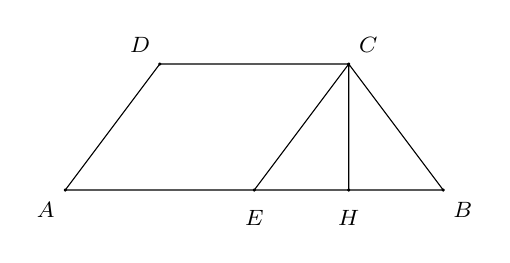
\begin{tikzpicture}[scale=.4,font=\footnotesize,line join=round,line cap=round,>=stealth]
\path
(0,0)coordinate(A)
(12,0)coordinate(B)
(9,4)coordinate(C)
(3,4)coordinate(D)
(6,0)coordinate(E)
(9,0)coordinate(H);
\draw (A)--(B)--(C)--(D)--(A) (C)--(E) (C)--(H);
\foreach \p/\g in {A/-135,B/-45,C/45,D/135,E/-90,H/-90}
\draw[fill=black] (\p) circle (1pt) node[shift=(\g:10pt)] {$\p$};
\end{tikzpicture}}
}
\end{ex}

\begin{ex}%[0H9C3-5]%[Dự án đề kiểm tra Toán 11 GHKII NH23-24- Tổng Nguyễn]%[THPT Đống Đa - Hà Nội]
Trong mặt phẳng $O x y$, cho hình thang $A B C D$ có đáy lớn $C D=3 A B, C(-3;-3)$, trung điểm của $A D$ là $M(3;1), S_{B C D}=18, A B=\sqrt{10}$ và đỉnh $D$ có hoành độ nguyên dương. Giả sử điểm $B(a;b)$. Tính $3 a-b$.
% \shortans[]{$-10$}
\loigiai{\immini{
Do $M$ là trung điểm $AD$ nên $\mathrm{d}(M,CD)=\dfrac{1}{2}\mathrm{d}(B,CD)$.  Diện tích tam giác $MCD$ là
\[S_{MCD}=\dfrac{1}{2}\cdot S_{BCD}=\dfrac{1}{2} \cdot 18=9. \qquad(1)\]
Vì $C(-3;-3)$ và $D$ có hoành độ nguyên dương nên đường thẳng $CD$ không thể vuông góc với trục $Ox$. Gọi $(x,y)$ là toạ độ điểm $D$. Khi đó $\vec{CD}=(x+3;y+3)$. Vì $x+3\ne 0$ nên đặt $k=\dfrac{y+3}{x+3}$.\\
Gọi $\vec{MN}$ thoả $\vec{MN}\perp \vec{CD}$ và $MN=CD$. Suy ra $\pm \vec{MN}=(y+3;-(x+3))$.\\
Ta có $\vec{MC} = (-6;-4)$\\
}{\begin{tikzpicture}[scale=.5,font=\footnotesize,line join=round,line cap=round,>=stealth]
\draw[->] (-4,0) --(0,0) node[above right] {\footnotesize $O$}-- (4,0) node[below] {\footnotesize $x$};
\draw[->] (0,-4) -- (0,7) node[left] {\footnotesize $y$};
\foreach \x in {-3,3}
\draw[shift={(\x,0)},color=black] (0pt,2pt) -- (0pt,-2pt) node[below] {\footnotesize $\x$};
\foreach \x in {-3}
\draw[shift={(0,\x)},color=black] (2pt,0pt) -- (2pt,0pt) node[below left] {\footnotesize $\x$};
\path
(0,0)coordinate(O)
(4.2,-3)coordinate(D)
(3,1)coordinate(M)
(-3,-3)coordinate(C);
\coordinate (A) at ($(D)!2!(M)$);
\coordinate (B') at ($(A)+(C)-(D)$);
\coordinate (B) at ($(A)!1/3!(B')$);
\foreach \p/\g in {A/90,B/90,C/-90,D/-90,M/0}
\draw[fill=black] (\p) circle (1pt) node[shift=(\g:3mm)] {$\p$};
\draw (A)--(B)--(C)--(D)--(A) (B)--(D) (M)--(C);
\end{tikzpicture}}
Khi đó $d(M,CD)=MC\cdot \left\|\cos \left( \vec{MC}, \vec{MN}\right)\right\| = MC \cdot \dfrac{|-6(y+3)+4(x+3)|}{\sqrt{(y+3)^2+(x+3)^2}}=MC\cdot \dfrac{|-6k+4|}{\sqrt{k^2+1}}$.\\
Ta có  $CD=3AB=3\sqrt{10}$.  Diện tích của tam giác $MCD$ 
\[S_{MCD}=\dfrac{1}{2}\cdot CD\cdot \mathrm{d}(M,CD)=\dfrac{3\sqrt{10}\cdot|6k-4|}{2\sqrt{k^2+1}} =\dfrac{3\sqrt{10}|3k-2|}{\sqrt{k^2+1}}.\qquad(2)\]
Từ (1) và (2), ta có
\[\dfrac{3\sqrt{10}|3k-2|}{\sqrt{k^2+1}}=9\Leftrightarrow \sqrt{10}|3k-2|=3\sqrt{{{k}^{2}}+1}\Leftrightarrow 81{{k}^{2}}-120k+31=0\Leftrightarrow \hoac{&k=\dfrac{1}{3}
\\&k=\dfrac{31}{27}.}\]
\begin{itemize}
\item Với $k=\dfrac{1}{3}$, ta có 
\[ CD=3\sqrt{10}\Leftrightarrow \sqrt{(x+3)^2+9\left(x+3\right)^2}=3\sqrt{10}\Leftrightarrow \hoac{&x=6 \Rightarrow D(6;0)\ (\text{nhận})\\&x=-12\Rightarrow D(-12;-6)\ (\text{loại}).}\]
Vì $M(3;1)$ là trung điểm của $AD$ nên
\[\heva{&x_A=2\cdot 3-6=0\\&y_A=2\cdot 1-0=2.}\]
Do đó $A(0;2)$.\\
Từ điều kiện $\overrightarrow{BA}=\dfrac{1}{3}\overrightarrow{CD}=(3;1)$. Gọi $B(m;n)$ khi đó
\[\overrightarrow{BA}=(3;1)\Leftrightarrow \heva{&0-m=3\\&2-n=1}\Leftrightarrow \heva{&m=-3\\&n=1.}\]\\
Do đó  $B(-3;1)$.
\item Với $k=\dfrac{31}{27}$ ta có 
\begin{eqnarray*}
& &CD=3\sqrt{10}\\
&\Leftrightarrow& \sqrt{(x+3)^2+\left(\dfrac{31}{27}x+\dfrac{4}{9}+3\right)^2}=3\sqrt{10}\\
&\Leftrightarrow& (x+3)^2=\dfrac{6561}{169}\\
&\Leftrightarrow& \hoac{&x=-\dfrac{120}{13}\ (\text{loại})\\&x=\dfrac{42}{13}\ (\text{loại}).}
\end{eqnarray*}
\end{itemize}
Do đó  $B(-3;1)$ thỏa yêu cầu đề bài.\\
Vậy  $3a-b=3(-3)-1=-10$.

}
\end{ex}


\begin{ex}%[VDC8-Phan Anh Tiến]%[1D2G2-6]
	Một nhóm gồm $5$ cô gái ký hiệu lần lượt là $G_1$, $ G_2$, $G_3$, $G_4$, $G_5$ và $12$ chàng trai. Có 17 chiếc ghế xếp thành hàng ngang. Người ta xếp nhóm người đã cho ngồi vào 17 chiếc ghế đó thỏa các điều kiện sau đây
	\begin{enumerate}[i)]
		\item Mỗi ghế có đúng một người ngồi.
		\item Thứ tự ngồi của các cô gái xét từ trái sang phải là $G_1$, $ G_2$, $G_3$, $G_4$, $G_5$.
		\item Giữa $G_1$ và $G_2$ có ít nhất ba chàng trai.
		\item Giữa $G_4$ và $G_5$ có ít nhất một chàng trai và nhiều nhất bốn chàng trai.
	\end{enumerate}
	Hỏi có bao nhiêu cách sắp như vậy?
	% \choice
	% {$\mathrm{C}_{17}^{5}$}
	% {$12!\cdot 5!\cdot 4!$}
	% {\True $1161\cdot 12!$}
	% {$\mathrm{A}_{18}^{4}$}
	\loigiai{Gọi $x_1$ là số chàng trai xếp trước $G_1$, $x_2$, $x_3$, $x_4$, $x_5$, $x_6$ lần lượt là số chàng trai xếp giữa $G_1$ và $G_2$, $G_2$ và $G_3$, $G_3$ và $G_4$, $G_4$ và $G_5$, sau $G_5$.\\
		Khi đó ta có hệ điều kiện sau   
		$$\heva{x_1+x_2+\cdots+x_6&=12\\x_i&\in\mathbb{N}\\x_2&\ge 3\\4\ge x_5&\ge 1.}$$
		Xét các trường hợp cụ thể sau
		\begin{itemize}
			\item [\textbf{TH1:}] $x_5=4$, phương trình viết lại thành $\left( x_1+1\right) +\left( x_2-2\right) +\left( x_3+1\right) +\left( x_4+1\right) +\left( x_6+1\right) =10$.\\
			Đặt $\left( x_1+1\right) =y_1$, $\left( x_2-2\right)=y_2$,  $\left( x_3+1\right)=y_3$, $\left( x_4+1\right)=y_4$, $\left( x_6+1\right)=y_6$. Ta được phương trình mới $y_1+y_2+y_3+y_4+y_6=10.$\\
			Xét dãy gồm $10$ số $1$, chọn $4$ trong $9$ vị trí giữa các số $1$ để đặt dấu cộng. Khi đó ta có một tổng theo thứ tự từ trái sang gồm $5$ số tự nhiên khác $0$ và tổng bằng $10$.\\
			Do đó có $\mathrm{C}_{9}^{4}$ bộ số $y_1,y_2,y_3,y_4,y_6$ thoả mãn yêu cầu.\\
			Suy ra số bộ nghiệm của hệ trong trường hợp này là $\mathrm{C}_{9}^{4}$.
			\item [\textbf{TH2:}] $x_5=3$, tương tự như trên ta có số nghiệm là $\mathrm{C}_{10}^{4}$.
			\item [\textbf{TH3:}] $x_5=2$, tương tự như trên ta có số nghiệm là $\mathrm{C}_{11}^{4}$.
			\item [\textbf{TH4:}] $x_5=1$, tương tự như trên ta có số nghiệm là $\mathrm{C}_{12}^{4}$.
		\end{itemize}
		Vậy số bộ nghiệm của hệ là $1161$.\\
		Tuy nhiên ta có thể hoán đổi vị trí sắp xếp của các chàng trai với nhau, do đó số cách sắp xếp thỏa yêu cầu đề bài là $1161\cdot 12!$. 
	}
\end{ex}
